\section{Method}
This section explains how the two parts of this thesis were executed. First, the Big Data-pipeline for the automatic collection of the tweets is described in further detail. Then, the way this generated data set is visualized is discussed. Lastly, the interview study in which laymen tested the prototype is further described. The full architecture of data collection and storage can be seen in \textbf{Figure \ref{fig:architecture}}.

\begin{figure}[htb]
    \fbox{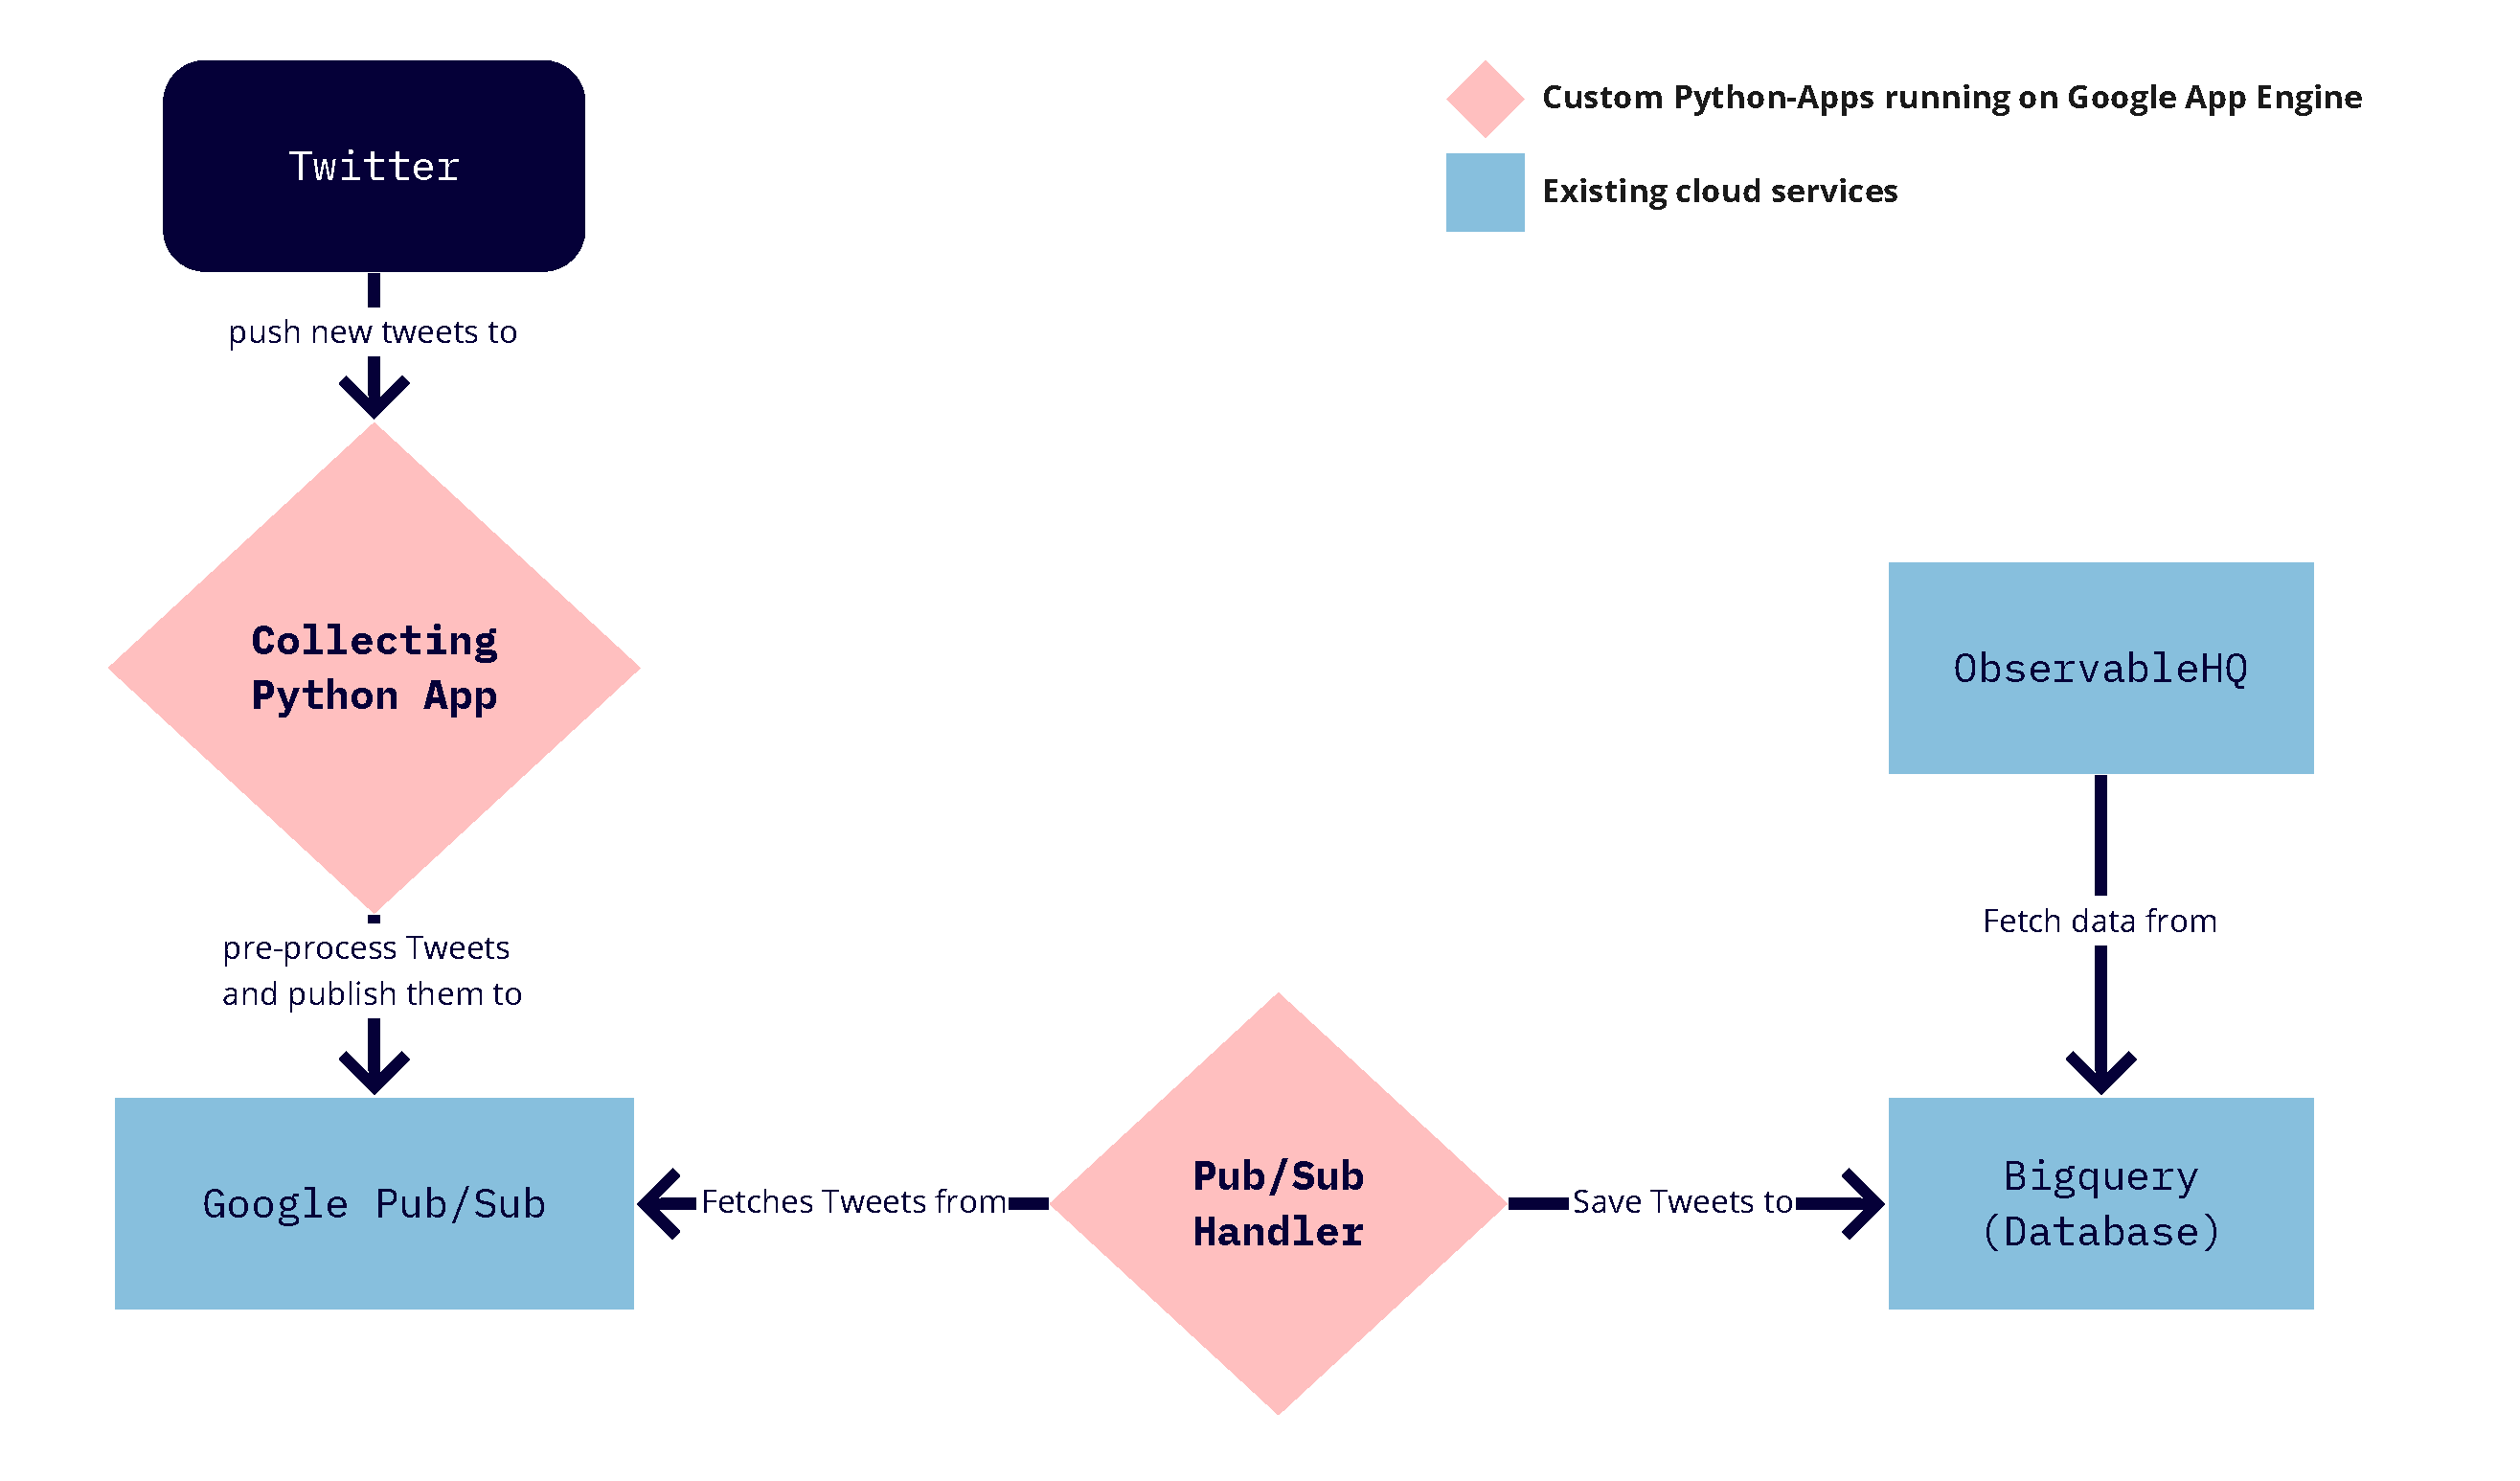
\includegraphics[width=\linewidth]{images/architecture.pdf}}
    \caption{The software architecture, showing how data collection, processing, storage, and visualization relate to each other.}
    \label{fig:architecture}
\end{figure}

\subsection{Data collection pipeline}
This section will go into further detail about which data was collected from Twitter and how this data was collected, prepared, and stored. Technical considerations about the collection and storage will also be discussed.

\subsubsection{Fetching the data from Twitter} \label{sec:fetchedData}
The application for collecting the tweets was written in Python 3 (\cite{10.5555/1593511}), the Twitter API was accessed using the package \emph{Tweepy} (\cite{roesslein2020tweepy}). Tweepy's connection to Twitter's Streaming API was used to collect all German-language tweets containing one or more of the keywords \verb+Corona, Covid-19, Covidioten, Distancing+.

From the returned Tweet Objects\footnote{The documentation on what data a Tweet Object contains can be found here: https://developer.twitter.com/en/docs/tweets/data-dictionary/overview/tweet-object (last visited on Oct. 13, 2020)} only a few data points were kept that seemed interesting before the data collection started. This has mainly ethical reasons (\cite{richards2014big}). The author of this study did not want to collect excessive personal data without good reason, even though this has become the norm for big data over the last decade. The following data points of a Tweet Object are processed further and eventually saved to a database:

\begin{itemize}
\item \textbf{The full text of the tweet.} This is mainly used for sentiment analysis and other natural language processing tasks.
\item \textbf{The timestamp of the tweet.} This is the exact date and time when the tweet was sent.
\item \textbf{The ID of the tweet.} This makes it easier to check for duplicates in the database. 
\item \textbf{The user name of the tweet author.} As discussed above, opinion leadership is also a phenomenon on Twitter. Collecting user names allows, e.g., to analyze which users tweet the most.
\item \textbf{The user's self-description.} Users on Twitter can enter a short description, the so-called \emph{bio}.
\item \textbf{The user's friend count.} This shows how many other accounts the user in question is following.
\item \textbf{The user's follower count.} This shows how many other accounts follow the user in question.\footnote{The definitions for friend- and follower count can be found here: https://developer.twitter.com/en/docs/accounts-and-users/follow-search-get-users/overview (last visited on Oct. 13, 2020)}
\item \textbf{The country from which the tweet was sent.} Twitter also offers coordinate-based geolocations, but choosing the country instead seemed to honor the user's privacy more.
\item \textbf{Whether the account is verified or not.} Accounts can be verified by Twitter, which means that they are run by the person who the account claims to be. Verified accounts are often influencers and have a lot of followers.
\item \textbf{The source of the tweet.} This shows if the tweet came from the web app, a desktop app, a mobile app, a 3rd party-application, or other sources.
\item \textbf{The calculated sentiment of the tweet.} The sentiment score, which represents how positive or negative a tweet is, is calculated during the pre-processing step. Later sections will go into more detail on how the sentiment is calculated.
\end{itemize}

%TODO: Add figure how the data was collected (it's in miro)

Twitter offers two different methods to automatically collect tweets:
\begin{enumerate}
    \item \textbf{Twitter's Archive API} allows users to automatically search for content in Twitter's archives. There are several levels of access to this API. The free tier gives access to data from the last seven days. Paid tiers give access to up to 30 days. Access is limited to 1\% of the global tweet volume at any time, no matter the tier. The API grants access to tweets on a randomized basis.
    \item \textbf{Twitter's Streaming API} works differently from this. Instead of accessing an asynchronous archive on Twitter's servers, the Streaming API pushes tweets that match the search criteria to an endpoint the moment a tweet is sent. The Streaming API does not grant access to tweets that were already sent before the collection started, though.
\end{enumerate}

For this study, the Streaming API was used as it gives the most complete data set on Twitter's free tier (\cite{brunsTwitterDataWhat2014}). It pushes (or streams) tweets that match the above-mentioned criteria to a specified endpoint the moment such a tweet gets sent on Twitter. %The alternative to the Streaming API is to access Twitter's archive, access to which is severely limited on the free tier of the Twitter API. Using the free tier, it is only possible to collect data from the last seven days, and even then the data set is not complete. Because of this, the Streaming API was used in this study.
%TODO: Grafik zur Erläuterung. Kann ja vermutlich ein einfaches Flussdiagramm sein: Python App (bekommt Tweets von) Streaming API (läuft auf) Docker-Container (schubst Daten nach) BigQuery

Using the streaming API had two downsides. First, the Python app that collected the tweets had to reliably run 24/7 over a prolonged time. The Streaming API streams the data as it comes in and does not save it on Twitter's network, which means that every tweet the Python app does not 'catch' immediately will be lost. Second, the data produced by the streaming API could only be analyzed after the collection ran for several days. This trade-off, and possible ways to circumvent it, will be further on page \pageref{sec:fixedDataSet}.

To ensure constant availability, the python application that connects to the Streaming API and processes the incoming tweets runs on Google's App Engine (\cite{googleAppEngineApplication2020}). App Engine is Google's high-reliability service for serverless cloud apps. Programmers can use App Engine to constantly run their apps on Google's servers, instead of hosting their servers.

Inside of App Engine, the Python app ran in a Docker Container (\cite{merkel2014docker}). Docker Containers bundle the operating system, dependencies, settings, and more. As Docker's documentation puts it,

\begin{quote}
    A [Docker] container is nothing but a running process, with some added encapsulation features applied to it in order to keep it isolated from the host and from other containers. One of the most important aspects of container isolation is that each container interacts with its own private filesystem; this filesystem is provided by a Docker image. \emph{An image includes everything needed to run an application} - the code or binary, runtimes, dependencies, and any other filesystem objects required. (\cite{dockerOrientationSetup2020}, emphasis by the author.)
\end{quote}

This combination of a highly reliable service and a fully independent container running the app made it easy to set up a serverless infrastructure with high availability.

\subsubsection{Processing the data during the collection}
Every time the Streaming API sent a tweet to the app collecting the data, a \emph{sentiment score} for the tweet text was calculated. This score between -1 and +1 indicates how negative or positive a tweet was written. To calculate the sentiment, the Natural Language Toolkit (NLTK, \cite{loper2002nltk}) was used. NLTK uses a dictionary-based approach for sentiment analysis. This means that NLTK uses a corpus that is coded with different sentiment scores (\cite{haselmayer2017sentiment}). Each word in this corpus is annotated with a score, based on how positive or negative a word is. The corpus for the sentiment analysis tool VADER (\cite{gilbert2014vader}), that can be viewed publicly on GitHub\footnote{https://github.com/cjhutto/vaderSentiment}, contains examples of how this works. A word like 'elegant', for example, gets assigned a score of 2.1; 'embarrassment' a score of -1.9. Using formulas that take additional factors, like negation ('not elegant') and boosting ('huge embarrassment') into account, these scores are used to calculate the overall normalized sentiment of the tweet which lays between -1 and 1.

Compared with machine learning-approaches, this approach has high precision, but low recall (\cite{sorokaBadNewsMad2015}). This means that the polarity of a sentiment as computed by NLTK is usually correct; however, many texts that do carry a specific sentiment are not recognized and marked as texts with neutral sentiments. Because of this possible drawback, machine learning-based approaches were also considered.

One powerful tool to calculate the sentiment of a text with a machine learning-based approach is Google's Natural Language Cloud API (\cite{googleSentimentAnalysisTutorial2020}). Using this API leverages the power of a well-trained machine learning model. As this API calculates the cost of analysis per document, and each tweet would have been a single, short document, this solution was deemed too expensive for this thesis. At the time of writing, processing the on average around 40,000 tweets that were collected daily would have summed up to costing 40€ per day for the sentiment analysis alone.

Another machine learning-based approach for calculating sentiments, based on Stanford NLP (\cite{stanfordnaturallanguageprocessinggroupSoftwareStanfordNatural}, was also considered for this study. This approach requires a second server that runs a Java application. This would have meant a second instance of Google App Engine, doubling the costs.

Considering that the goal of this study is to test how laymen work with the data set, and not a scientific analysis of the discussion about the coronavirus in the German Twittersphere, the dictionary-based approach was chosen to keep down the costs. %maybe re-formulate it so it doesn't sound as lazy?

\subsubsection{Storing the pre-processed tweets}\label{sec:storage}
Tweets collected via the Streaming API are bundled to batches of 100. These batches then get published as a message to a \emph{Pub/Sub Topic}. Pub/Sub allows asynchronous messaging between services that \emph{produce} events, like in this case the app that collects the tweets, and services that \emph{process} events, in this case the database which stores the collected tweets (\cite{googleWhatPubSub2020}).
This approach has multiple advantages. For one, the database connection does not need to be open constantly. This makes the pipeline more robust: If the database connection is closed---for whatever reason---the messages published to the pub/sub topic are saved for up to 30 days. Once the database connection is re-established, the messages get ingested and the tweets are added to the database.

It also allowed for some early experimentation with the table schema for the SQL table. Pub/Sub could be configured so that already acknowledged messages stay in the system and can be fetched again. This meant that even though the table schema was constantly reset in the first couple of days of data collection, the data was not lost and could simply be re-fetched again.

The tweets are stored in a \emph{Google BigQuery} database, a serverless data warehouse that allows fast analysis of large amounts of data (\cite{googleBigQueryCloudData2020}). Using such a serverless data warehouse guaranteed high reliability and easy access to the database. \emph{Google Firebase} was also considered as data storage (\cite{googleCloudFirestoreFirebase2020}). As Firebase is a NoSQL database, the database queries would have been easier to write: Instead of using SQL, standard JavaScript could have been used. This would have resulted in easier queries, as JavaScript features, like method chaining, would have been available.

Seeing that the SQL-based BigQuery is better equipped to handle large amounts of data, this solution was chosen in the end. Using BigQuery meant that the queries needed to be written in SQL, a language infamous for its complicated semantics (\cite{slutz1998massive}). BigQuery was chosen over other SQL databases, like SQLite or Postgres, because it is also a Google service like App Engine. This meant that authentication between the script collecting the tweets and the database did not have to be implemented. BigQuery can also be directly connected to a Pub/Sub-Topic using Google DataFlow. Because the data was additionally processed, saving it was handled in a dedicated script. 

\subsection{Building the web-app to present the interactive visualizations}
To visualize the data from the Streaming API, both Python libraries like ggplot (\cite{wickhamGgplot2ElegantGraphics2016}) and JavaScript libraries like D3 (\cite{bostockD3JsDataDriven}) and VegaLite (\cite{uwidlVegaLiteHighLevelGrammar}) were evaluated. To make the prototype as accessible as possible, a JavaScript-based library was chosen, as JavaScript is a popular web technology. A web page is easier to access to laymen than a Python-based app, as there is no need to install additional tooling. And even though Python scripts, including visualizations, can be embedded easily on the web now, choosing a native web technology that could be run on most devices seemed like the right approach.

Ultimately, D3 was chosen as a visualization framework. VegaLite is an opinionated framework which chooses many defaults for the user, while D3 is unopinionated. This means that the visualizations are harder to code but more versatile.

Early prototypes of the tool used a Svelte-based web page to show the visualizations. The final tool, however, was written in Observable\footnote{https://observablehq.com}. Observable is a JavaScript-based notebook that, similarly to Jupyter Notebooks, combines code, output, and explanatory text. The notebooks allowed for quick iteration of the code, while its web-based nature also satisfied the requirement of being easily accessible without the need to download and install additional software.

\subsubsection{Filtering and fetching the data from the database}
While D3 can work with raw data input and perform, e.g., filtering operations on these inputs, data operations were performed directly in the database using SQL queries. This decision was made because the final data set was almost 1GB big. Relying on D3 for filtering and aggregating the data would have meant that every time a user opens the tool, they would have to wait for the whole data set to finish downloading before they could use the tool itself. Using SQL queries instead meant that a lot fewer data had to be sent to the tool. Instead of downloading the full 997MB of the data set, the query results were only about 10KB big which greatly improved performance.

%To explore the data set of collected tweets, users can have three additional filters that they can use
Users could explore the data using different filters. This corresponds to the second part of Shneiderman's Visual Information Seeking Mantra \say{zoom and filter} (\cite[337]{shneidermanEyesHaveIt1996}). Users could use three different filters:

\begin{enumerate}
    \item A word-filter that allows users to search the database for tweets including a specific word
    \item A toggle whether to include retweets in the data set
    \item A toggle whether to include neutral tweets in the data set, \emph{neutral} meaning tweets with a sentiment between -0.3 and +0.3 on a scale from -1 to 1 %TODO: write in related work about this
\end{enumerate}

The final layout of the toggles can be seen in \textbf{Figure \ref{fig:volume_barchart}}.

The toggles to include retweets and neutral tweets in the data set changed the visualizations immediately, whereas the word-filter initiated a new database query. The idea behind this was that users are likely to look for a specific topic and then want to explore how this topic is presented in the data set.

One possible scenario is that users want to research the public's general opinion on masks. They then enter the keyword \emph{mask} into the search field and can then explore this topic further. The first version of the dashboard made a new database call every time one of the toggles was clicked. This became an issue already in early stages of creating the prototype: The delay caused by the database call made it difficult to compare the visualizations with the different filters, e.g., to compare how the graph looks with or without retweets included.

Because of this, data fetching was rewritten before the user tests started. Every time a user filters for a new word, the tool fetches the data for the four different filter permutations: the full data set, the data set without retweets, the data set without neutral tweets, and the data set without retweets and neutral tweets. If the user then toggles additional filters, the corresponding pre-fetched data set gets immediately visualized instead of fetching a new data set from the database.

\subsubsection{Visualizing the tweet volume over time}
The final prototype that was tested included two different visualizations:

\begin{enumerate}
    \item \textbf{A visualization of the tweet volume over time:} Users can explore how many tweets were sent per day. When filtering for a word, users can see how many of the tweets per day contained the word they searched for. They can also toggle a normalized view which shows the percentage of tweets containing the search word, rather than the absolute number. The tested version of this visualization can be seen in \textbf{Figure \ref{fig:volume_barchart}}.
    \item \textbf{A visualization of the sentiment over time:} Using this visualization, users can explore if and how the public perception of a topic changed over time. This visualization also offers two views. The default view shows two lines: One line displays the sentiment for the tweets containing the search word, the other line displays the sentiment for the tweets \emph{not} containing the search word. A toggle shows only the daily average of all tweets instead, regardless of the search word. The tested version of this visualization can be seen in \textbf{Figure \ref{fig:sentiment_linechart}}.
\end{enumerate}

\begin{figure}[htb!]
    \fbox{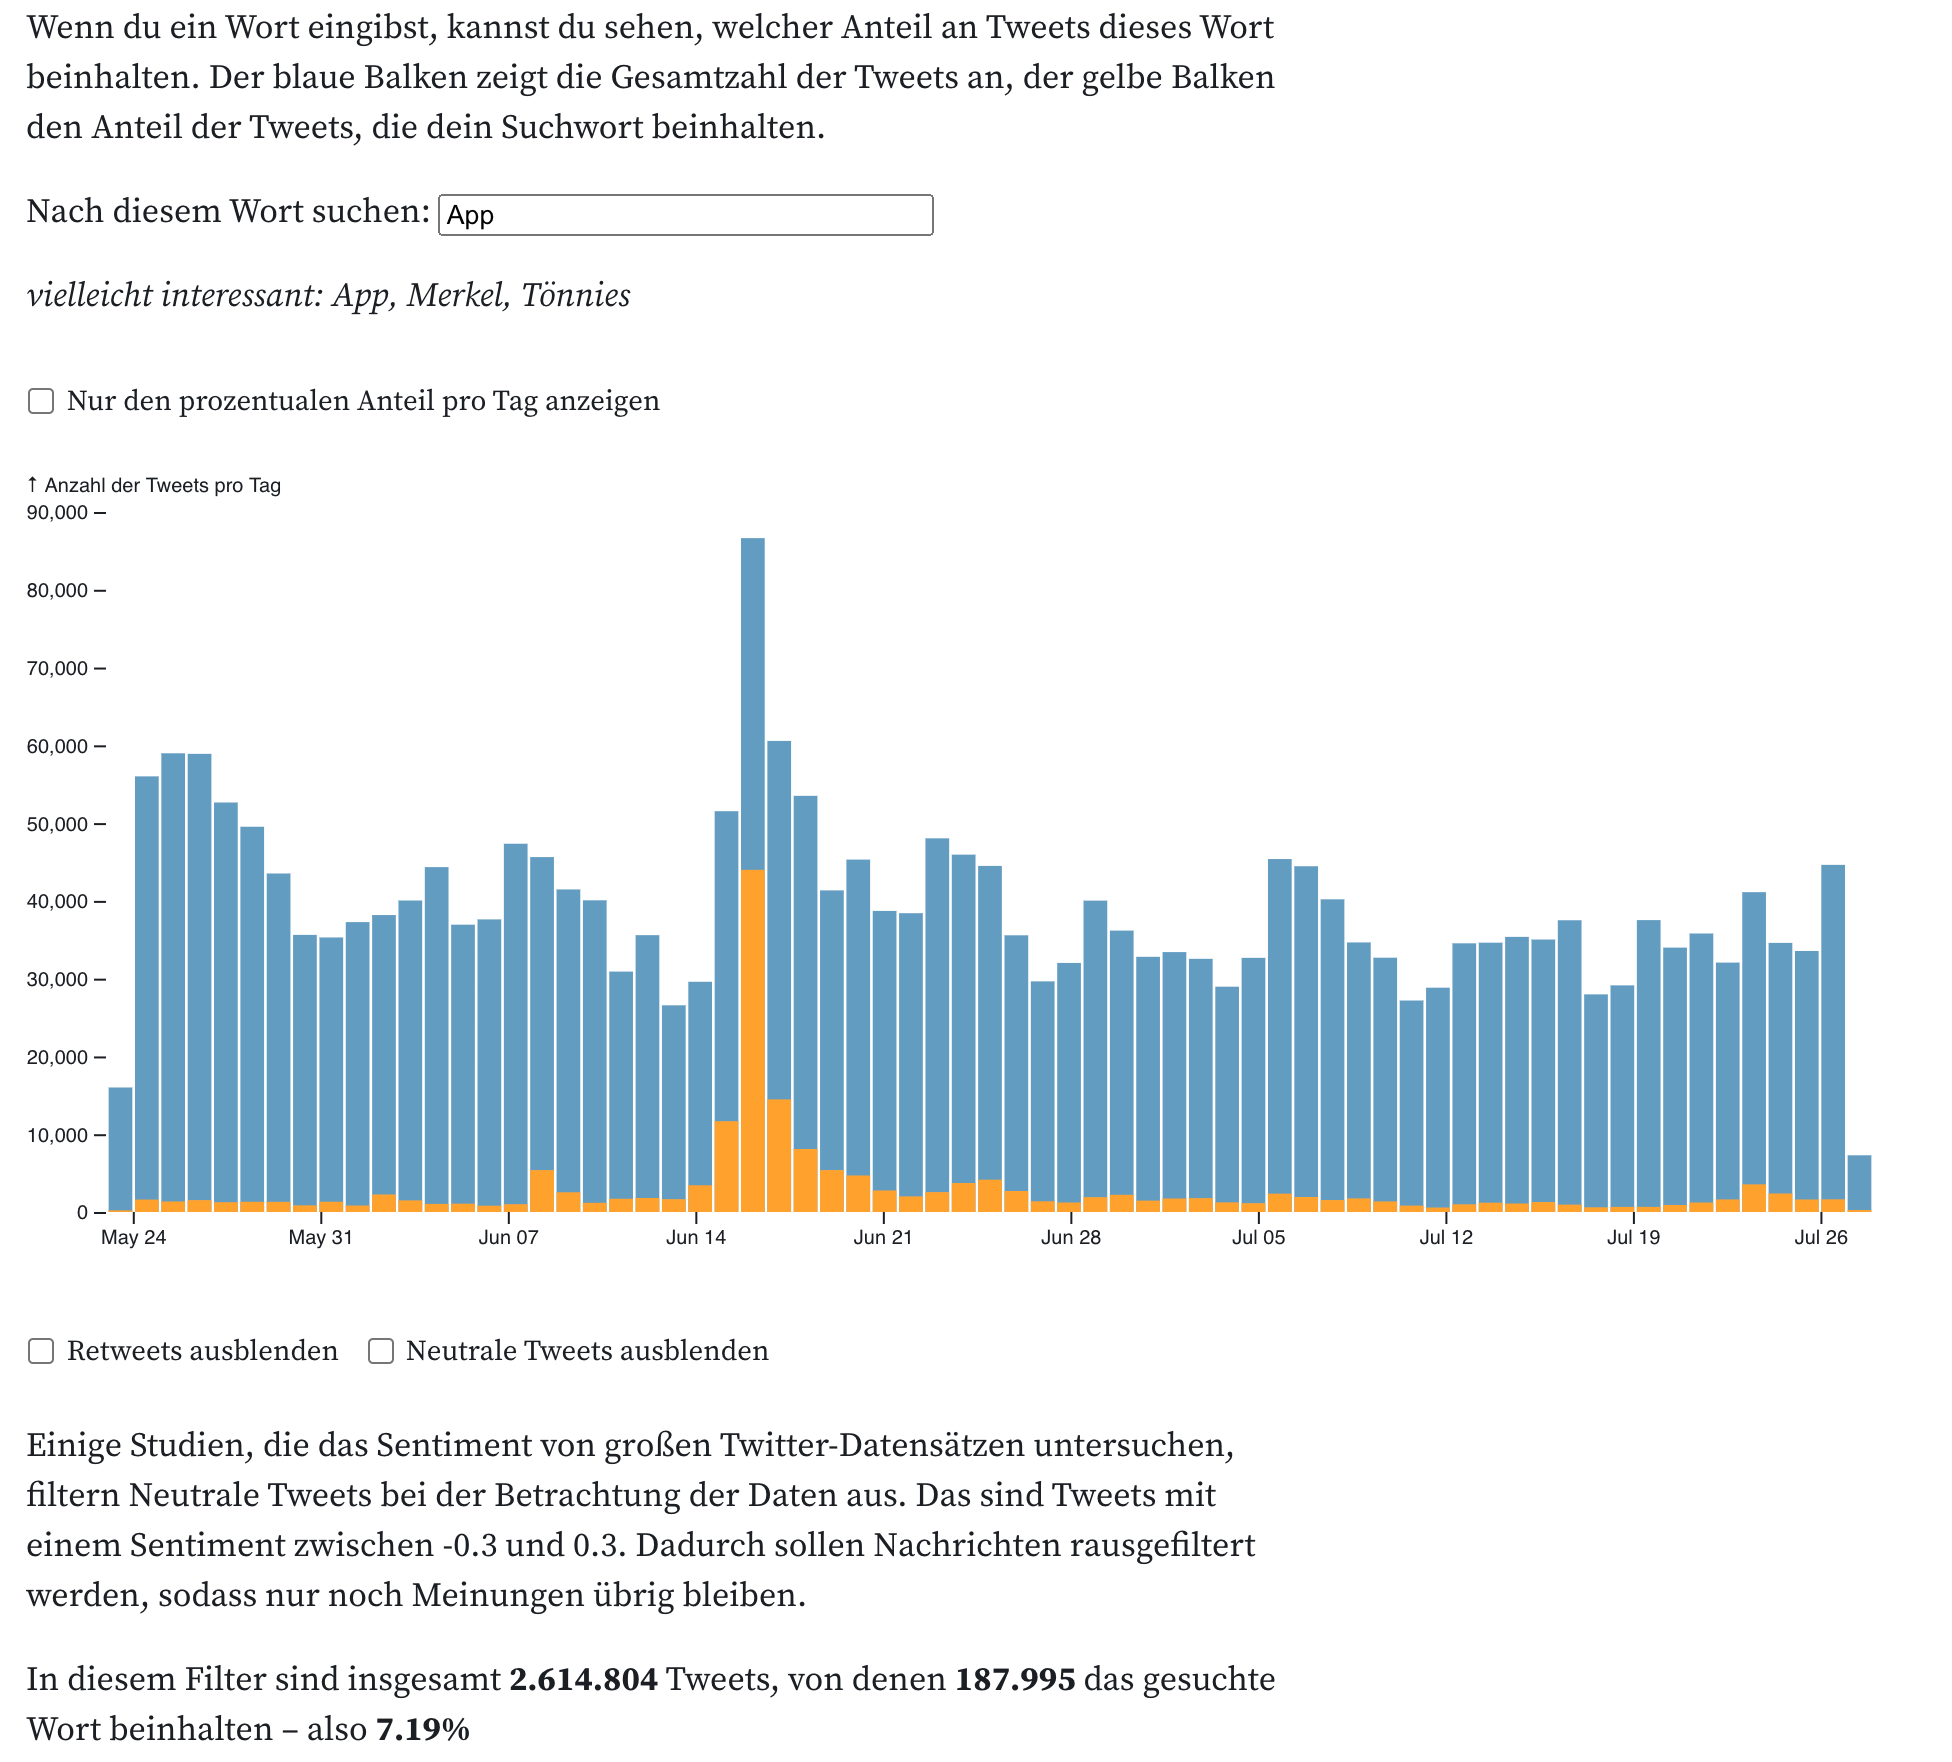
\includegraphics[width=\linewidth]{images/final_prototype_volume.png}}
    \caption{The final prototype version of the volume chart including explanatory texts. This example shows the distribution of the word \emph{App}. The spike in activity is on June 15th, the day the Corona Warnapp was released.}
    \label{fig:volume_barchart}
\end{figure}

Time series---meaning the development of certain aspects over time---were chosen as the primary visualization type because they are one of the most common visualizations (\cite{heerTourVisualizationZoo2010}). Choosing a common visualization aids laymen to read and interpret the data more easily (\cite{bornerInvestigatingAspectsData2016}), whereas more complicated visualizations can be difficult to understand for those people. As a result, the development of certain aspects of the data set \emph{over time} was chosen as the primary type of information that the visualizations should convey.

\begin{figure}[h!tb]
    \fbox{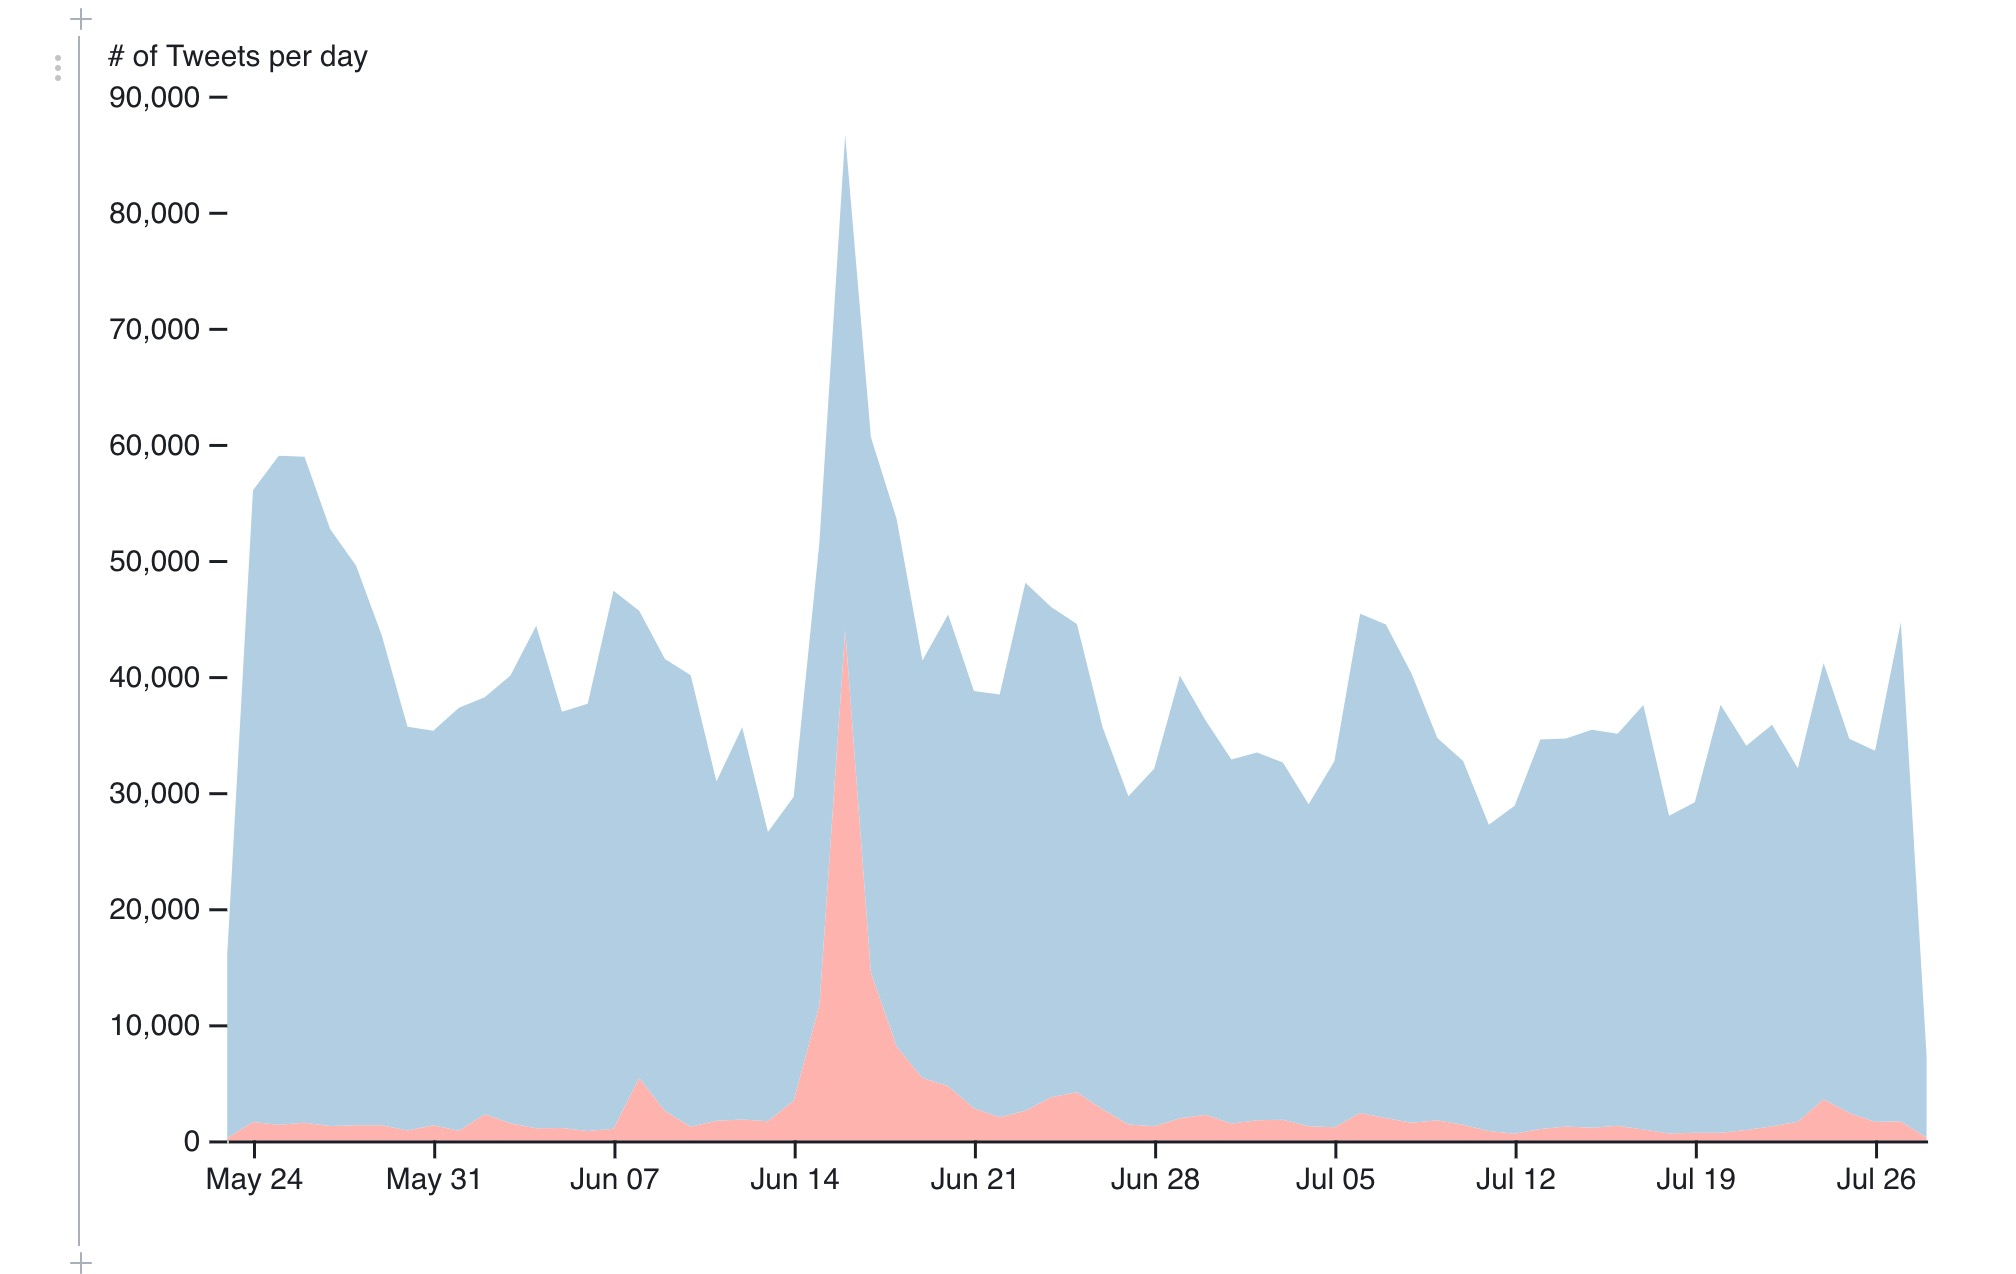
\includegraphics[width=\linewidth]{images/volume_areachart.jpg}}
    \caption{The first iteration of the daily tweet volume as shown in an area chart. This example shows the distribution of the word \emph{App} in red. The blue area shows the number of total tweets.}
    \label{fig:volume_areachart}
\end{figure}

To visualize the tweet volume over time, both an area chart and a bar chart were considered. Line charts and area charts are both common visualizations to show how something changed over time. Stock prices, for example, are usually shown as a line chart. An area chart is a line chart with its areas filled, which can be seen in \textbf{Figure \ref{fig:volume_areachart}}. The filled area was used to indicate how many tweets contained the search word. However, visualizations that use line or area charts to show development over time usually show data over a wider time range. For example, stock prices, which are often visualized using line charts, are usually shown over several years, as the general trend is more interesting than specific data points.

The data set for this study, however, spanned only around two months. Because of this, the chart was changed to a bar chart, as seen in \textbf{Figure \ref{fig:volume_barchart}}. Bar charts cannot show information as concise as line charts or area charts, but they make it easier to find and compare specific days. This could be especially interesting for data sets that span a couple of months, instead of several years.

Using Chrome's responsive design inspector, the bar chart was pre-tested across multiple device sizes and appeared to be usable even on 11-inch displays without horizontal scrolling. The final user tests all used the bar chart visualization for the tweet volume.

The final visualization also contained labeled axes. The x-axis showed dates, with ticks every 7 days. The y-axis, labeled \say{↑ Anzahl der Tweets pro Tag} (\emph{↑ Number of tweets per day}), showed numbers between 0 and 90,000 on a linear scale, with ticks every 10,000 tweets. The domain of the y-axis remained the same, even when the data set was filtered and therefore shrank. It was programmed to lie between 0 and the highest value in the biggest data set so that the biggest data set still fit into the visualization.

This ensured that datasets remained easily comparable when different filters were applied. If the domain would have changed to always lie between 0 and the highest value in the \emph{current} data set, it would have meant that the maximum of the smallest data set would have been visualized with a bar exactly as high as the maximum of the biggest data set---even though it would have been a difference of around 90,000 tweets vs. 11,000 tweets. The effect of fixing the domain can be seen in \textbf{Figure \ref{fig:variableVsFixedDomain}}.

\begin{figure}[h!tb]
    \fbox{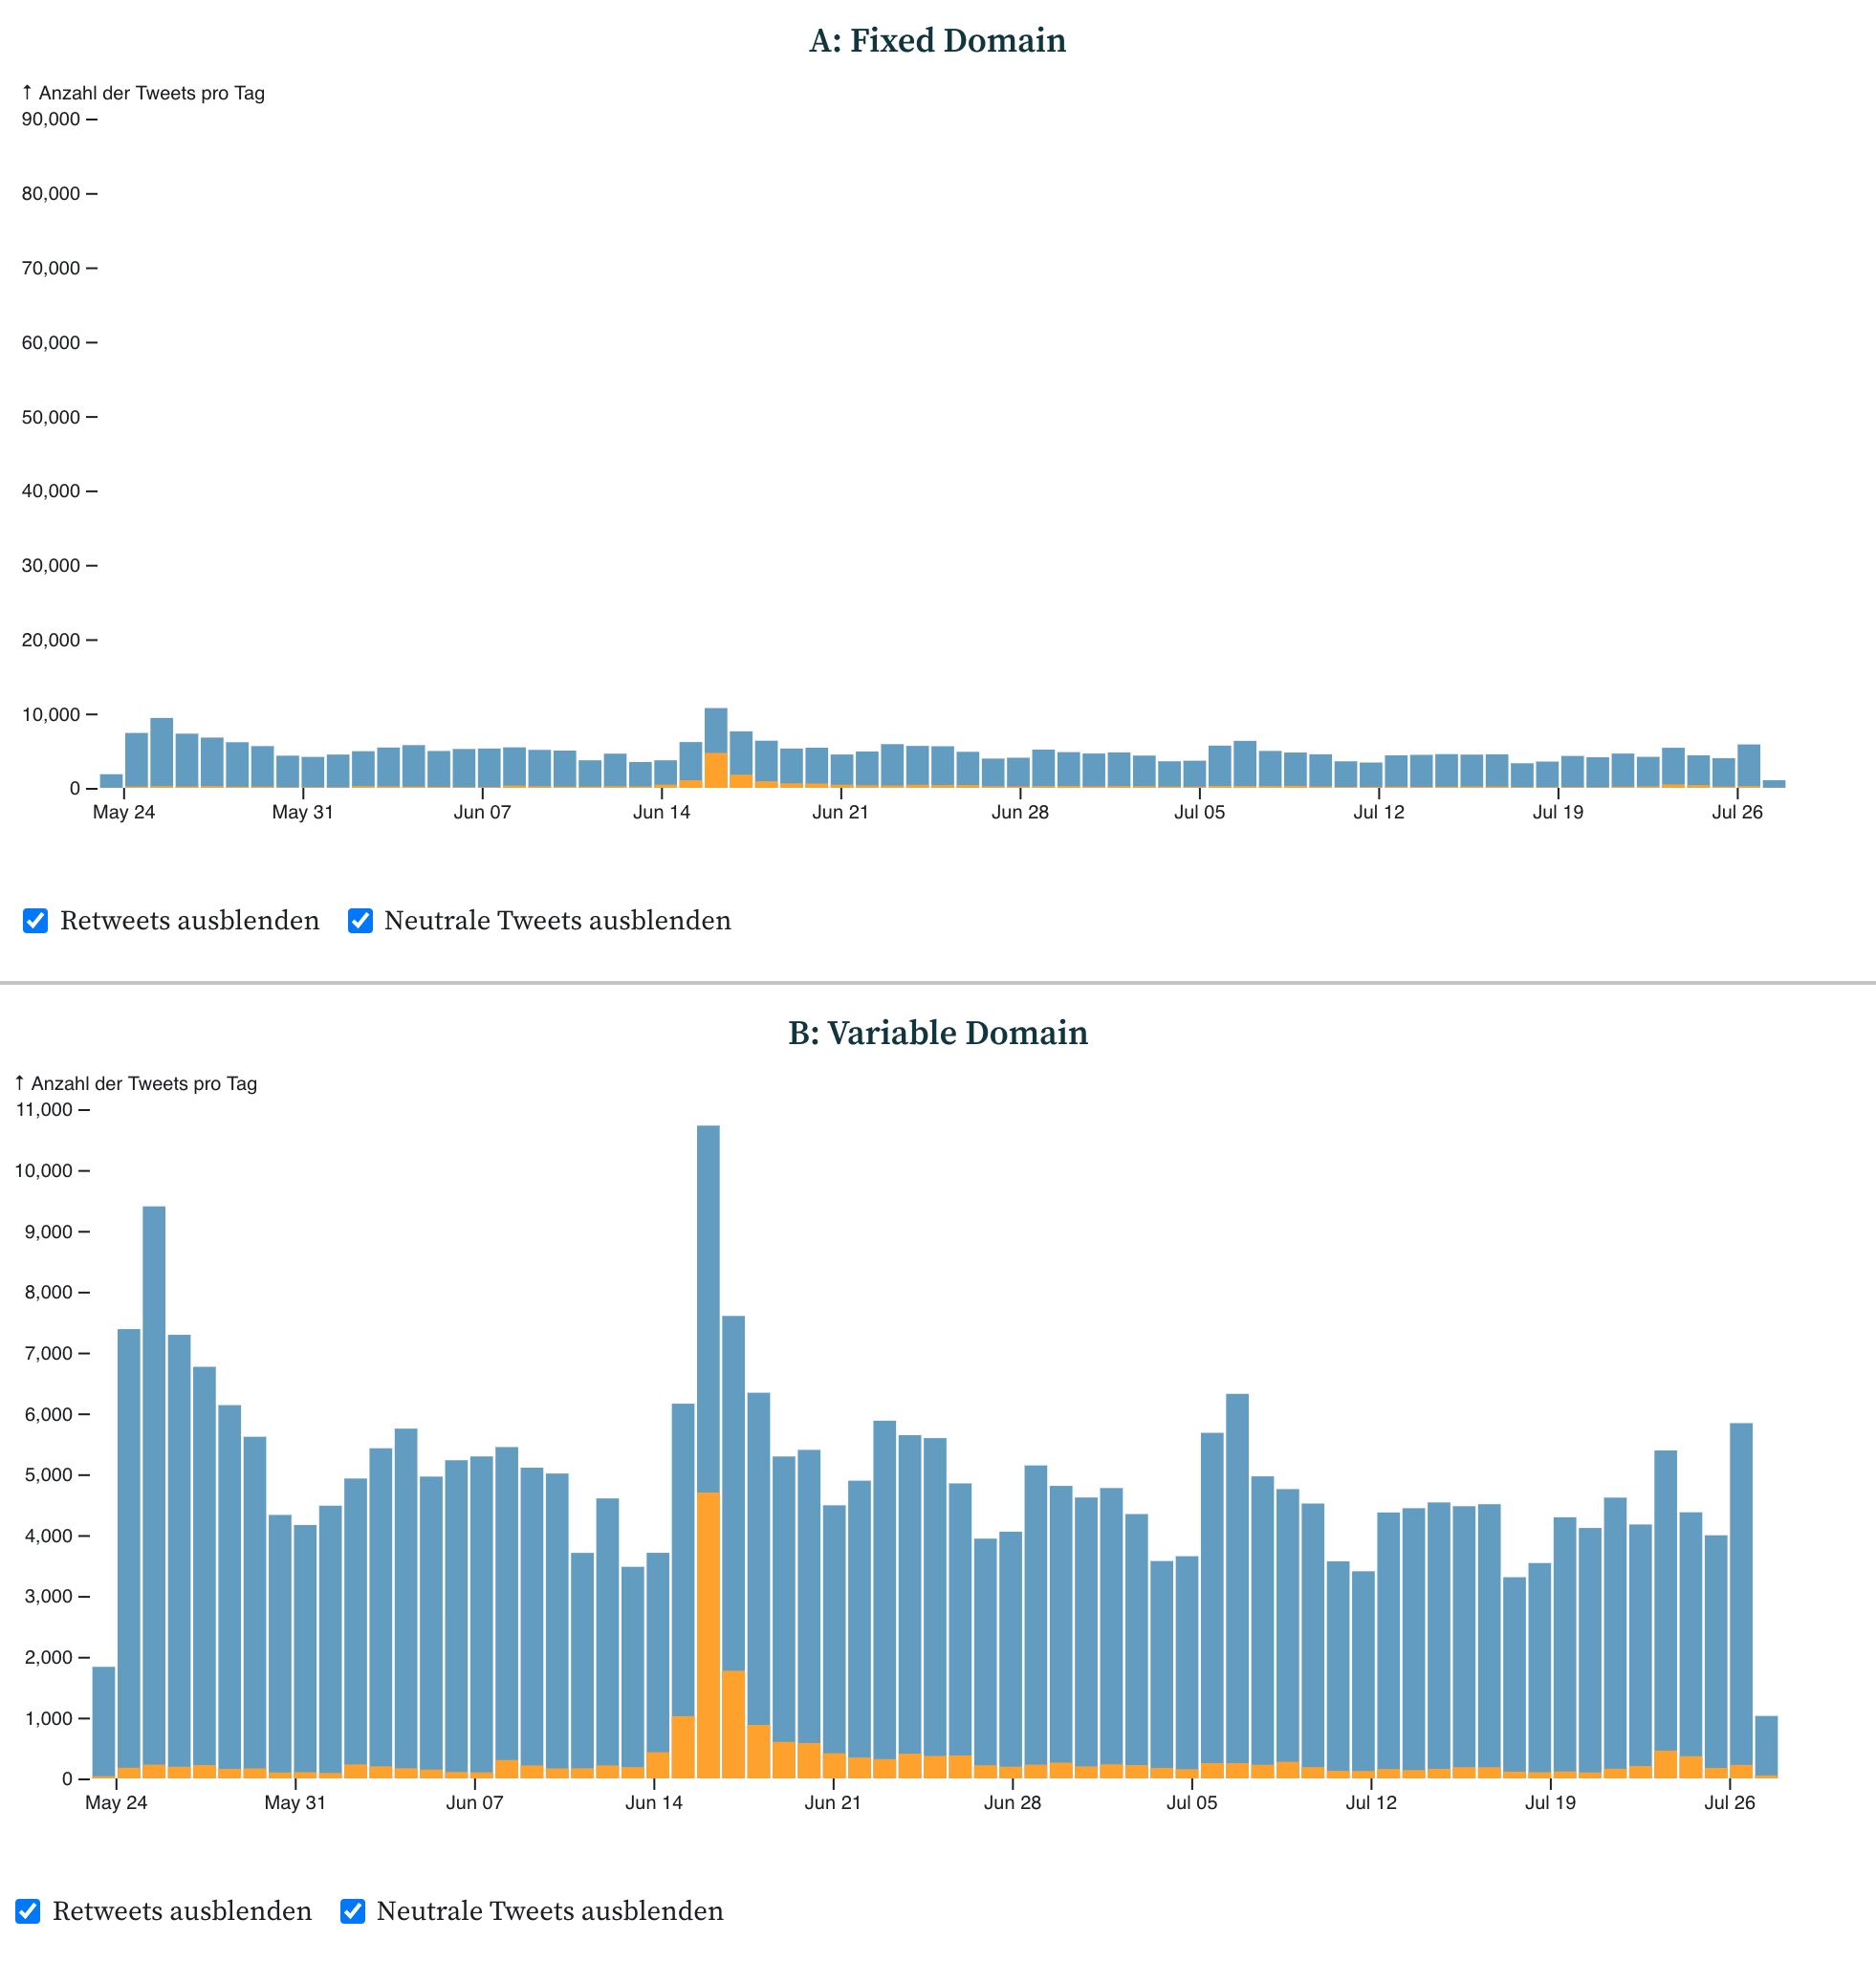
\includegraphics[width=\linewidth]{images/variableVsFixedDomain.png}}
    \caption{Showing the effect of a fixed and a variable domain. Both visualizations show the distribution of the word \emph{App}, and both have the same filters applied.}
    \label{fig:variableVsFixedDomain}
\end{figure}

The bar chart showing the tweet volume over time also contained tooltips, satisfying \citeauthor{shneidermanEyesHaveIt1996}'s requirement for \emph{details-on-demand} (\cite{shneidermanEyesHaveIt1996}). These tooltips were realized by adding title attributes to the div-containers that create the bars. The code for this can be seen in \textbf{Figure \ref{code:details_title}}. By hovering over the bars, this title attribute was shown---this is the default behavior for every modern browser. The title attribute contained the date of the currently hovered bar, the total number of tweets on this day, the number of tweets containing the search word on this day, and the percentage of tweets containing the search word on this day. As the line chart is not built using a single div per day, but rather from one SVG-line, this solution could not be used in the chart showing the development of the sentiment over time. This limitation will be further discussed in Section \ref{fw_tooltips}.

\begin{figure}[h!]
    \begin{verbatim}
svg.append("rect:title")
    .text(
        d =>
        `${formatTime(d.date)} | ${d.query_count} von ${
            d.total_count
    } Tweets (${(d.percentage * 100).toFixed(1)} %)`
);
    \end{verbatim}
    \caption{The code that adds the date, the number of words containing the search word, the total number of tweets, and the percentage of words containing the search word to the bin of every day. The detailed data were added as an unformatted string to the title attribute.}
    \label{code:details_title}
\end{figure}

\subsubsection{Visualizing the average daily sentiment over time}
The visualization which shows the development of the average daily sentiment is a line chart (see Figure \ref{fig:sentiment_linechart}). Its domain ranges from -1 to +1.

\begin{figure}[htb!]
    \fbox{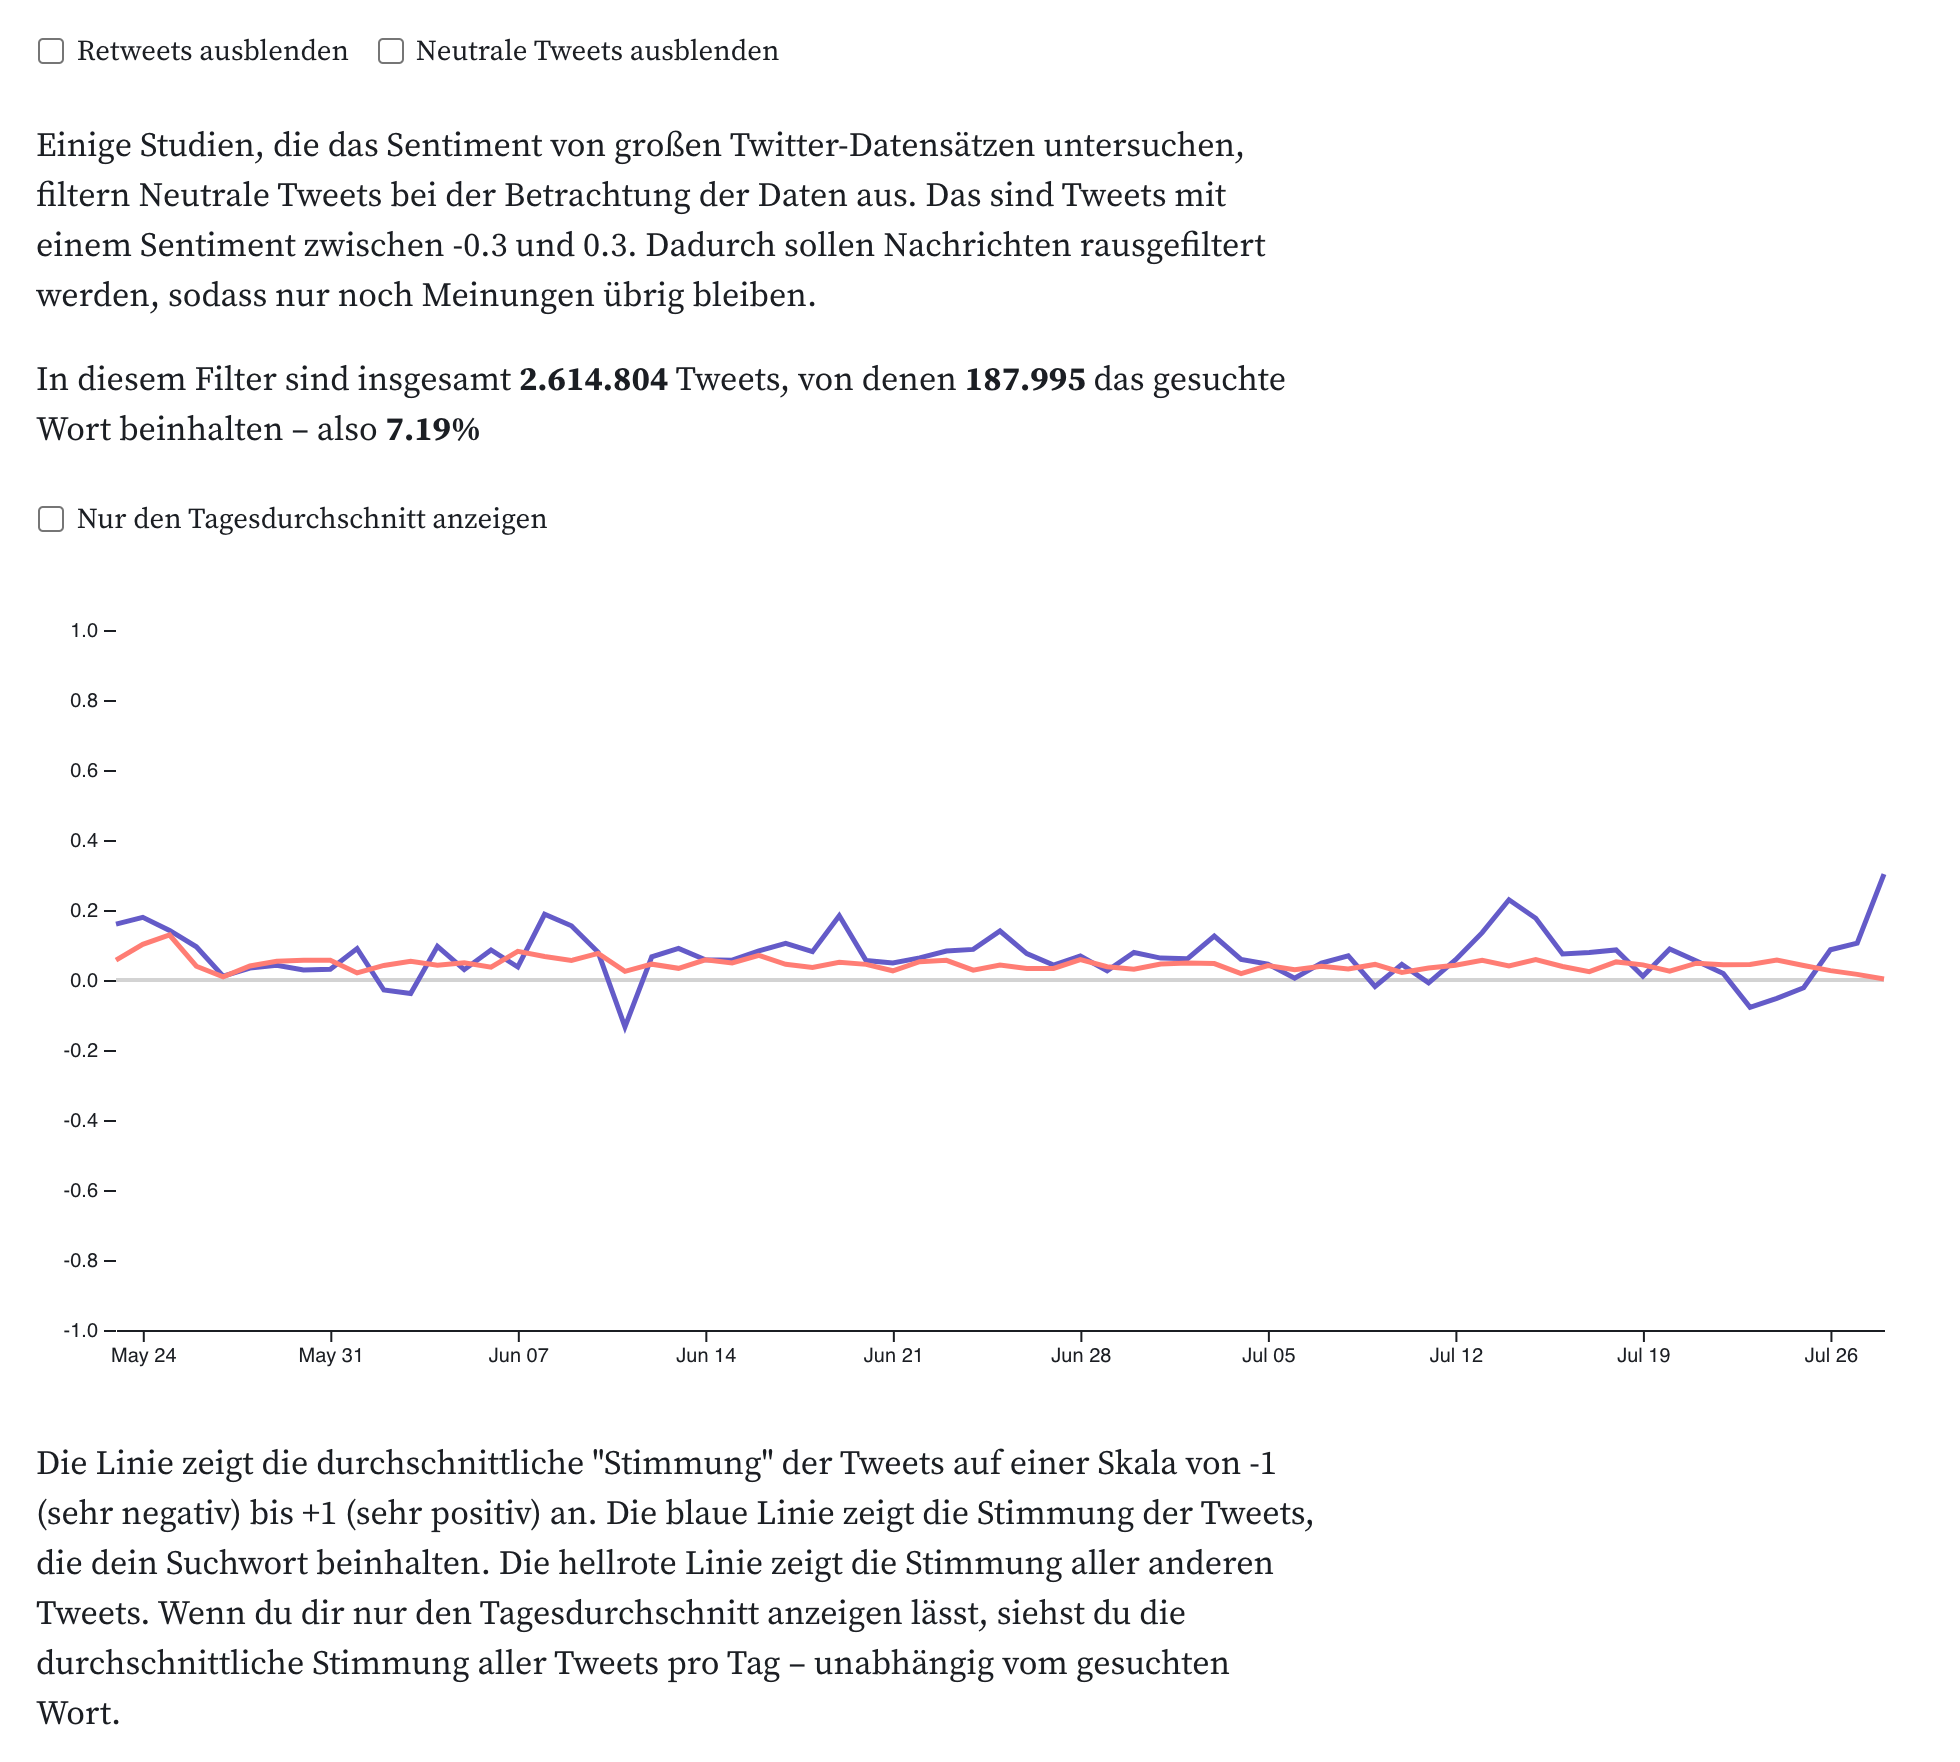
\includegraphics[width=\linewidth]{images/final_prototype_sentiment.png}}
    \caption{The final prototype version of the sentiment chart showing the average sentiment per day. The blue line shows the average sentiment of tweets containing the word \emph{App}, the red line shows the sentiment of tweets not containing this word.}
    \label{fig:sentiment_linechart}
\end{figure}

In this visualization, users can toggle between two view modes. The default mode shows the daily average sentiment of the tweets containing the search word as a blue line and the daily average sentiment of tweets \emph{not} containing the word as a red line. Users can also toggle to only see the average sentiment without any word-filters applied. This lets them, e.g., see the influence of neutral tweets or retweets on the whole data set.

The two visualizations share the same three aforementioned filters. Consequently, both visualizations share the same data set which could make it easier for participants to mentally connect them. At the same time, placing the filter possibilities at the top of the Observable notebook means that the visualizations are affected by filters that are not in their immediate neighborhood. As this trade-off was tested in the user study, it will be further discussed later in this work.

Explanatory texts for the visualizations were written and placed below the visualizations. This was done so that users are first confronted with the visualization and have the chance to find out what is displayed by themselves. Should they need further assistance, they could read the text below the visualization. Presenting the visualizations and the explanations in this order allows participants to try and form an understanding of the charts before and then test their assumptions against the explanation below.

The explanatory texts contained information about what kind of data was displayed, and what the different parts of the chart meant. They also included the explanation of which color coded which information in the visualizations.

\subsection{Testing the dashboard}
The user tests of the dashboard were testing two things: how users explore the data set using the dashboard, and how easily they can read the two visualizations. To test this, a guide for a semi-structured interview was prepared (\cite[315ff.]{schnell1999methoden}). This guide can be found in the appendix of this work.

The user test consisted of two parts. After a brief introduction to the topic of this master thesis and a quick overview of the data set, participants got around five minutes to explore the dashboard in any way they wanted. During this time, they were already asked to think aloud.

After this phase of free exploration, the participants were asked to solve four tasks in total, each with increasing difficulty. These tasks were designed to check the participants' ability to properly read the data visualizations. Again, participants were asked to think aloud while solving the tasks.

\begin{itemize}
    \item Task 1 was to find out on which day most tweets were sent. This task could be solved by finding the highest bar in the bar chart. It didn't matter which word was entered in the word filter as participants were asked to find the highest \emph{total} number of tweets, which can always be seen in blue (see \textbf{Figure \ref{fig:volume_barchart}}). Participants should toggle both neutral tweets and retweets to show up in the data set. After finding the highest bar, participants could hover over it to find the date in the tooltip. This type of task is one that, according to \citeauthor{northMeasuringVisualizationInsight2006}, does not generate a lot of insight. The goal of this task was to get the participants used to both the visualization and to thinking aloud, and to give them an immediate sense of achievement after solving this task.
    \item Task 2 was to find out on which day most tweets were sent about Dr. Drosten, who is known for communicating openly about his coronavirus studies (\cite{henleyCoronavirusMeetScientists2020}). This search term was used to see if the participants could figure out that the search is, in fact, a filter. Only very little results were found typing in \say{Dr. Drosten}. Participants had to search for \say{Drosten} instead. This task also aimed to find out whether participants understand the difference between the day with the absolute highest number of tweets and with the relative highest number, compared to the total number of tweets that day.
    \item Task 3 was to identify the sentiment about Dr. Drosten when the neutral tweets were filtered out. This task tested two things: first, if the quick filters were recognized as such, and if their job was clear. Second, the participants' ability and willingness to discuss ambiguous results were tested. The sentiments of tweets about Dr. Drosten changed significantly over time, with various peaks in both positive and negative sentiment as seen in \textbf{Figure \ref{fig:sentiment_drosten_noneutral}}. Thus, there was no definite answer to the question. Participants had to read the data carefully, interpret it, and voice their train of thought.
    \begin{figure}[htb]
        \fbox{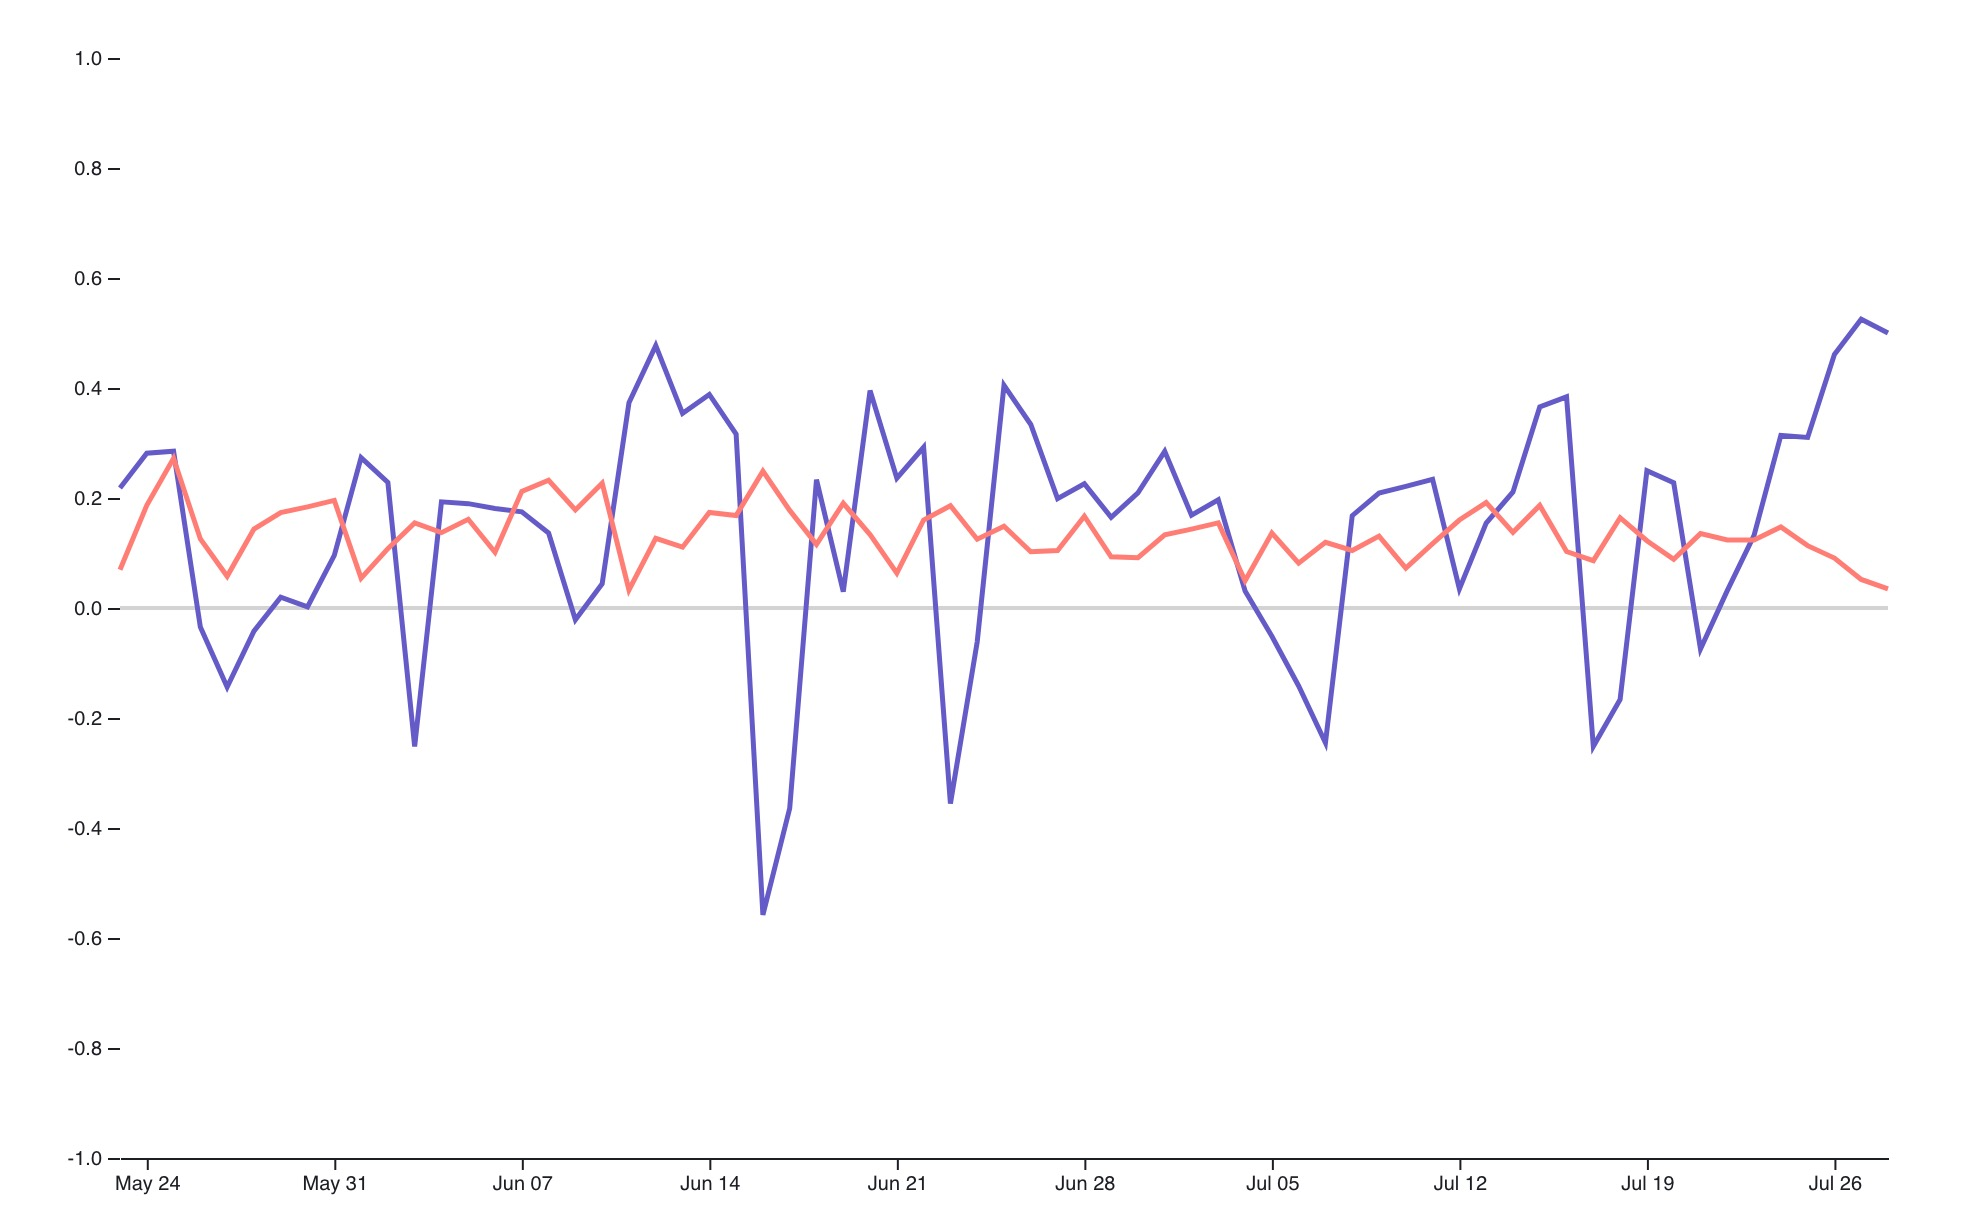
\includegraphics[width=\linewidth]{images/sentiment_drosten_noneutral.jpg}}
        \caption{The daily average sentiment of tweets containing the word \emph{Drosten}, without neutral tweets.}
        \label{fig:sentiment_drosten_noneutral}
    \end{figure}
    \item Task 4 was another task to test the participants' ability and willingness to discuss their findings. According to \citeauthor{northMeasuringVisualizationInsight2006}, this ability is an indicator to measure the insight users gain from a visualization (\cite{northMeasuringVisualizationInsight2006}). For this final task, participants were asked to find out how retweets influence the overall sentiment of the German twitter discussion about Covid-19. To solve this task, participants had to observe the influence the retweet-filter had on the sentiment graph and discuss this change. As in task 3, there is no definite right or wrong answer.
\end{itemize}

After the participants had completed the four tasks, a retrospective interview was conducted. The retrospective interview asked participants about their experience working with the tool and solving the tasks. Questions that arose during testing were also asked in the retrospective interview instead of during testing itself. Participants were further asked to report whether they had any questions in mind that they thought they should be able to answer using the dashboard.

Due to the ongoing Covid-19 pandemic, the interviews were conducted with the online video conference system Zoom\footnote{https://zoom.us}, rather than in person. Conducting the interview using Zoom had both advantages and disadvantages. On the one hand, Zoom allowed the recording of both the audio, the screen, and the participants' webcam, which made transcribing easier. Participants could also take part in the study from their own home, rather than having to travel to a prepared test room. This made it possible to ask participants who did not live in Aachen to take part in the interviews.

On the other hand, even though Zoom does not require a lot of effort to set up, this meant that people without access to an internet-capable device could not participate in the study. Also, less tech-savvy people could have been hindered from participating in the study because they didn't want to or didn't know how to install Zoom and join the video conference.

The recorded Zoom meetings were later transcribed to a reading version. After this, the transcriptions were coded based on Mayring's approach to qualitative content analysis (\cite{mayring2010qualitative}). For this, an inductive-deductive approach was used. Categories were derived from the material and sorted into two primary categories: \say{Motivationsfaktoren} (\emph{motivational factors}) and \say{Hemmfaktoren} (\emph{hindering factors}), based on whether the finding motivated the participants to use the tool or hindered their exploration. Then, more categories were created based on the contents of the interviews. The codebook, including anchor examples, will be discussed in the results section. 

The last part of the interview was a screening survey via Google Forms\footnote{https://forms.google.com}. Participants were asked to fill out this survey without supervision by the interviewer. Using Google Forms allowed the participants to fill out the questionnaire and send it to the interviewer in an already anonymized form. The questionnaire contained questions about age, gender, and Twitter usage of the participants.
